\section{Reducing the Model to One Half}

\Citeauthor{akyuz2022} pointed out in their master thesis, that the model satisfies the property in \Cref{equ:yunus.property.symmetry}.
This means, that there is some symmetry in the model.
In the following, I will reduce the model to only $\theta \mapsto F(\theta) \mod \pi$ and observe what happens in the thin area explored above.
\begin{align}
    F(\theta + \pi) & \equiv F(\theta) + \pi \mod 2 \pi \label{equ:yunus.property.symmetry}
\end{align}

Now, something interesting happens.
\Cref{fig:yunus.pi.2d.full} shows a 2D-scan of the same area that is depicted in \Cref{fig:yunus.2pi.2d.full}.
You can see that the thin areas now have a different color from the bigger areas.
This means that the period of the cycle or cycles in that area now have a higher period.

\begin{figure}
    \centering
    \includegraphics[width=0.6\textwidth]{98_Yunus_modpi/2D_Period/result.png}
    \caption{2D Scan of Halved Original Model}
    \label{fig:yunus.pi.2d.full}
\end{figure}

It is not immediately clear, what is happening.
Looking at the cobwebs helps.
\Cref{fig:yunus.pi.CobwebA2} shows the cycle before the thin area with period 6.
It has period 6 which is exactly one-half the cycle in the full model at the same parameter values for $E_0$ and $\chi_0$, since it is just one-half of the model.
Its symbolic sequence is $\L^3\R^3$.
The cycle that is stable after the thin area, displayed in \Cref{fig:yunus.pi.CobwebD2}, has the symbolic sequence $\L^2\R^4$.
So the move of one pint of the cycle to the other branch happens still.

But in the middle, there are not two cycles coexisting, but one cycle with double the period.
\Cref{fig:yunus.pi.CobwebB2,fig:yunus.pi.CobwebC2} show this cycle.
Its symbolic sequence is $\L^3\R^3\L^2\R^4$ and its rotation number is $\frac{12}{2}$.
The rotation numbers of the cycles outside the thin area in \Cref{fig:yunus.pi.CobwebA2,fig:yunus.pi.CobwebD2} are both $\frac{6}{1}$.
This looks like period-adding since we have the concatenation of $\L^3\R^3$ and $\L^2\R^4$, as well as the Farey-adding of the rotation numbers $\frac{6}{1} \oplus \frac{6}{1} = \frac{12}{2}$.
But on closer inspection, there is no further period-adding on either side of the thin area.

The reason we have coexistence in the full model and something different in this reduced model is that the cycle in the full model starts on either the first or the second rotation of $\L^3\R^3\L^2\R^4$ in the first half of the full model.
In the second half, it will have to behave like the other rotation.
For example, if the cycle starts on $\L^3\R^3$, in the full model this will translate to $\A^3\B^3$.
Then the cycle will have to behave like the second rotation in the right half of the model.
The second rotation is $\L^2\R^4$ which translates to $\C^2\D^4$ in the full model.
Concatenating both halves of the cycle in the full model will yield $\A^3\B^3\C^2\D^4$.
Analogous, starting on the second rotation $\L^2\R^4$ will yield the second cycle in the full model $\A^2\B^4\C^3\D^3$.

\begin{figure}
    \centering
    \begin{subfigure}{0.4\textwidth}
        \centering
        \includegraphics[width=\textwidth]{98_Yunus_modpi/Period6/Cobweb_A2/result.png}
        \caption{Before the thin area begins}
        \label{fig:yunus.pi.CobwebA2}
    \end{subfigure}
    \begin{subfigure}{0.4\textwidth}
        \centering
        \includegraphics[width=\textwidth]{98_Yunus_modpi/Period6/Cobweb_B2/result.png}
        \caption{After the thin area begins}
        \label{fig:yunus.pi.CobwebB2}
    \end{subfigure}
    \begin{subfigure}{0.4\textwidth}
        \centering
        \includegraphics[width=\textwidth]{98_Yunus_modpi/Period6/Cobweb_C2/result.png}
        \caption{the thin area ends}
        \label{fig:yunus.pi.CobwebC2}
    \end{subfigure}
    \begin{subfigure}{0.4\textwidth}
        \centering
        \includegraphics[width=\textwidth]{98_Yunus_modpi/Period6/Cobweb_D2/result.png}
        \caption{After the thin area ends}
        \label{fig:yunus.pi.CobwebD2}
    \end{subfigure}
    \caption{Cobwebs of Halfed Original Model}
\end{figure}
